\documentclass[11pt,a4paper]{article}
\usepackage[T1]{fontenc}
\usepackage[utf8]{inputenc}
\usepackage[margin=1in]{geometry}
\usepackage{amsmath,amssymb,amsthm}
\usepackage{mathpartir}
\usepackage{stmaryrd}
\usepackage{booktabs}
\usepackage{tabularx}
\usepackage{array}
\usepackage{enumitem}
\usepackage{listings}
\usepackage{xcolor}
\usepackage[expansion=false]{microtype}
\usepackage{tikz}
\usetikzlibrary{arrows.meta,positioning,fit,calc}
\usepackage[htt]{hyphenat}
\usepackage[hidelinks,pdftitle={Bytecode, or the normal form? The interpreter between K1NDL1NG and CampF1R3}]{hyperref}
\setlength{\emergencystretch}{3em}

\newcommand{\code}[1]{\texttt{#1}}
\newcommand{\Kind}{\textsc{K1ndl1ng}}
\newcommand{\Camp}{\textsc{CampF1R3}}
\newcommand{\Rhobots}{\textsc{Rhobots}}
\newcommand{\Bell}{\textsc{B3ll0ws}}
\newcommand{\MUST}{\textsc{must}}
\newcommand{\MUSTNOT}{\textsc{must not}}
\newcommand{\SHOULD}{\textsc{should}}
\newcommand{\SHOULDNOT}{\textsc{should not}}
\newcommand{\MAY}{\textsc{may}}
\newcommand{\enc}[1]{\llbracket #1 \rrbracket}
\newcommand{\cmp}[1]{\llparenthesis #1 \rrparenthesis}
\newcommand{\rr}{\rightharpoonup}
\newcommand{\Norm}{\code{Norm}}

\theoremstyle{definition}
\newtheorem{definition}{Definition}[section]
\newtheorem{requirement}[definition]{Requirement}
\newtheorem{decision}[definition]{Decision}
\newtheorem{obligation}[definition]{Obligation}
\newtheorem{remark}[definition]{Remark}
\newtheorem{criterion}[definition]{Criterion}
\theoremstyle{plain}
\newtheorem{proposition}[definition]{Proposition}
\newtheorem{lemma}[definition]{Lemma}

\lstset{
  basicstyle=\ttfamily\footnotesize,
  columns=fullflexible,
  keepspaces=true,
  breaklines=true,
  frame=leftline,
  framesep=6pt,
  xleftmargin=8pt,
  rulecolor=\color{black!30},
  showstringspaces=false,
}

\title{\textbf{Bytecode, or the normal form?}\\[1mm]
\large An analysis of the two designs for the interpreter\\
between \Kind{} and \Camp\\[2mm]
\normalsize Design analysis v0.1}
\author{F1R3FLY.io}
\date{17 September 2026}

\begin{document}
\maketitle
\begin{abstract}
\noindent
\Camp{} specifies a store and stops; \Kind{} specifies a parser and a normaliser
and stops. Between them sits an \emph{executive}, whose two unspecified pieces
are a matcher and an interpreter. This note analyses one question about the
interpreter: should it execute a bytecode compiled from the normal form, or
execute the normal form itself? The question turns out to be less symmetric
than it looks. Reflection --- the $*@P\equiv P$ law that distinguishes rho from $\pi$ ---
means arbitrary terms arrive at run time in process position, so a bytecode machine
for this calculus contains a term interpreter or a run-time compiler as a
component rather than as an alternative (Section~\ref{sec:refl}). The
normal-form encoding is already a flat, tag-dispatched, length-delimited byte
string, so the distance between the two options is not representation but
explicit control flow --- of which the kernel, having no conditionals, has none
(Section~\ref{sec:already}). And the store's channel identity is the encoding
itself, which forbids a compiled form from ever being a key unless the compiler
is proved canonical (Section~\ref{sec:identity}). The recommendation is to
interpret the normal form, with a prepared-continuation cache that captures the
one benefit a bytecode would have delivered, behind a backend seam that leaves
the other option open (Section~\ref{sec:rec}). The measurement that would
overturn the recommendation, and the two conditions under which it expires, are
stated (Sections~\ref{sec:measure}--\ref{sec:change}).
Key words \MUST, \MUSTNOT, \SHOULD, \MAY{} are used in the sense of RFC~2119.
\end{abstract}
\tableofcontents
%======================================================================
\section{The question}\label{sec:q}

\subsection{The hole both specifications leave}

The two specifications in \code{publications/campf1r3} are deliberately
incomplete in the same place. \Camp{} v0.1 is ``the RSpace with everything that
is not the store removed'': it holds data and continuations at channels, it
fires one matching step per cut, and it lists parsing, normalisation,
substitution and evaluation among its non-goals. \Kind{} v0.2 supplies the two
of those that are pure functions of a term --- text to tree, tree to normal form
--- and lists \emph{reduction in any form} among its non-goals, adding that ``a
term here is data''. Its Section~3.3 names what is missing:

\begin{quote}\small
Data and continuations at channels, the cut \dots \Camp. Spatial match of a
pattern against a datum \dots the kernel matcher. Choosing what runs, firing
it, and the substitution that follows \dots \emph{the interpreter}. Wiring,
policy, scheduling, presentation \dots the executive.
\end{quote}

\noindent
Its open decision~(8) says only that the interpreter ``needs only \code{-norm}
and a store''. This note is about what runs inside it.

\subsection{Two options}

\begin{description}[leftmargin=2.4em,style=nextline]
\item[Option~A --- the bytecode machine.] A compiler $\cmp{-}$ takes a normal
form to an instruction stream for an abstract machine with a program counter, an
operand stack and a constant pool. Sequences of local instructions terminate in
instructions that call \code{produce} and \code{consume}. The executive runs the
machine; the machine talks to \Camp.

\item[Option~B --- direct interpretation.] The executive walks the normal form
itself: it dispatches on the constructor of each top-level parallel component,
calls the store, applies the substitution that a comm result licenses, and
re-enters. No representation exists between \code{k1ndl1ng-norm} and
\code{campf1r3-core} other than the one \Kind{} already defines.
\end{description}

\noindent
Option~A has a pedigree in this programme. The March 2026 architecture for a
rholang~1.2 bytecode interpreter put the usual operations on ground types onto
lightweight stack machines, arranged for sequences of ground instructions to
terminate in operations against RSpace, and carried a proof sketch that the
compiler is fully abstract. That document is the best statement of the case for
Option~A, and Section~\ref{sec:A} takes its design as the reference shape.
The claim of this note is not that the design was wrong, but that its principal
premise --- a rich layer of ground computation between communications --- is
absent from the kernel that \Camp{} serves, and that three properties of
\emph{this} pair of specifications tilt the balance further.

\subsection{What is not at stake}

Neither option touches the surface syntax, the tree, the normaliser, the
encoding $\enc{-}$, the content hash, the store interface, the determinism
profiles or the wire format. Both options are strictly downstream of
$\enc{-}$, and both leave \Kind{} and \Camp{} exactly as specified. The
question is confined to one crate that does not yet exist. This is worth
stating plainly, because it bounds the cost of getting the answer wrong: the
decision is reversible, and Section~\ref{sec:rec} recommends keeping it so.

\subsection{Criteria}\label{sec:crit}

The options are judged on seven axes, in the order of the weight given to them
here.

\begin{center}
\begin{tabularx}{\linewidth}{@{}l>{\raggedright\arraybackslash}X@{}}
\toprule
Axis & Question\\
\midrule
C1 Semantic burden & What must be proved that would not otherwise have to be?\\
C2 Identity discipline & Does it disturb the property that channel identity is
$\enc{-}$, and that equal terms have equal hashes?\\
C3 Reflection & How does it handle a term that arrives at run time and must then
be run?\\
C4 Performance & What fraction of the loop does it actually address?\\
C5 Budgets & Code size, dependency allowlist, \code{wasm32} parity, absence of
recursion and of \code{unsafe}, totality on hostile input.\\
C6 Consumers & What does it cost the three executives --- headset, browser,
node --- and the editor?\\
C7 Extensibility & What happens when the kernel grows: K2 guards, then the
\code{Expr} layer, then full f1r3lang?\\
\bottomrule
\end{tabularx}
\end{center}

\noindent
C1 and C2 lead because both specifications are unusually proof-shaped: \Camp{}
rests on the bialgebra reading of RSpace and carries an explicit obligation that
its comm rules are single reduction steps, and \Kind{} calls
Requirement~2.7 --- $\enc{P}=\enc{Q}$ iff $P\equiv Q$ --- ``the single most
load-bearing property in this document''. An interpreter that disturbs either is
expensive in the currency this programme actually spends.

%======================================================================
\section{What the interpreter does}\label{sec:work}

\subsection{The loop}

Fix the instantiation from \Kind{} Section~7: $C$ is a name in normal form
(a quoted \Norm, a free level, or an unforgeable), $A$ is \Norm, $P$ is a
\Norm{} whose free variables and wildcards are binding sites, and
$K=\code{Cont}\{\code{body}:\Norm,\ \code{binders}:\code{u16}\}$. Content hashes
are \Kind's memoised hashes of $\enc{-}$. With that fixed, the executive's whole
run loop is the following.

\begin{lstlisting}
// one round, from a comm result kappa = (k, pi, g, pats, (b_i, a_i, pi_i))
1. sigma  := bindings b_i, in binder order                     // executive
2. body'  := k.body.substitute(&sigma)                         // k1ndl1ng-norm
3. body'  := renormalise(body')       // order, encode, hash   // k1ndl1ng-norm
4. for p in body'.top_level() {                                // executive
5.     match p.shape() {
6.         Nil            => drop,
7.         Send{..}       => space.produce(chan, args, persist)?,
8.         Receive{..}    => space.consume(group, pats, cont, persist, peeks)?,
9.         New{k, body}   => mint k names, substitute, spawn body,
10.        Eval{name}     => splice the term the name quotes,   // reflection
11.    }                                                        // each may
12. }                                                           // return Some(kappa')
13. re-issue per the persistence contract; loop.
\end{lstlisting}

\noindent
Steps 9 and 10 are where the kernel's two remaining constructors are handled;
step~13 is \Camp's re-issue contract, which exists so that every operation
remains a single cut and the store returns at most one comm result per call.
That is the entirety of execution at K0 and K1. There is no arithmetic, no
comparison, no collection operation, no method call, no conditional and no
loop that is not a recursive process.

\subsection{Where the time goes}

Let $m$ be the node count of the continuation body, $s$ the mean encoded subterm
size, $w$ the width of a parallel composition, $\ell$ the join width, $n_c$ the
number of data at a channel, and $\mu$ the cost of one matcher call.

\begin{center}
\begin{tabularx}{\linewidth}{@{}llll>{\raggedright\arraybackslash}X@{}}
\toprule
Step & Owner & Cost & Bytecode helps?\\
\midrule
1 bindings & executive & $O(\ell)$ & no\\
2 substitute & \code{-norm} & $O(m)$ & no --- a machine substitutes too\\
3 renormalise & \code{-norm} & $O(m+\sum w\log w\cdot s)$ & no --- identity discipline\\
4--5 dispatch & executive & $O(w)$ & \textbf{yes} --- this line only\\
7--8 store op & \Camp & $O(\log n_c)$ bookkeeping & no\\
7--8 matching & matcher & $O(\ell\,\mu\max_i n_{c_i})$ & no\\
\bottomrule
\end{tabularx}
\end{center}

\noindent
\Camp's own performance section says the worst cases ``are dominated by $\mu$,
the spatial matcher'', and that the store's overhead per matcher call is $O(1)$.
\Kind{} budgets normalise-and-hash at $\ge 100$\,MiB/s of encoding. Between
them, steps 2, 3 and the matcher account for the arithmetic of the loop, and a
bytecode machine addresses none of them. It addresses step~4--5: the
structural dispatch over an arena of \code{u32}-indexed nodes.

\begin{remark}[Amdahl, stated early]\label{rem:amdahl}
Whatever fraction of the run loop is spent on structural dispatch is the
\emph{ceiling} on Option~A's improvement, before the cost of compilation is
subtracted. Section~\ref{sec:measure} makes measuring that fraction the first
task of the executive's phase, and proposes a threshold at which this note's
recommendation should be revisited.
\end{remark}

\subsection{The kernel has no ground layer}\label{sec:noground}

The rholang~1.2 bytecode design opened with the shape of program it was designed
for:
\[
  \code{for}(\,v_1\leftarrow u_1\ \&\ \cdots\ \&\ v_m\leftarrow u_m\,)\ \{\
     \code{let}\ w_1=e_1(v_i)\ \cdots\ w_n=e_n(v_j)\ \code{in}\ x!(w_1,\dots,w_n)\ \}
\]
The payload of that design is the middle: a run of ground expressions $e_k$ ---
arithmetic, comparisons, string and collection methods --- evaluated on a
thread-local stack, with a single store interaction at each end. Compiling that
run to a flat instruction stream is a textbook win, and the argument is sound.

The kernel \Camp{} serves has no middle. \Kind{} Section~2.4 puts ground
literals of every sort, collections, methods, \code{contract}, \code{match},
\code{select}, \code{let}, \code{if}/\code{else}, bundles, \code{VarRef}, the
logical connectives and simple types explicitly out of scope; each is a reserved
word producing a level diagnostic. K2 adds \code{where} guards over the
\code{rho-pure-eval} subset, behind a cargo feature, off by default, possibly
deferred to v1.1, and \Kind{} is clear that no crate of its family evaluates
them.

\begin{center}
\begin{tabularx}{\linewidth}{@{}l>{\raggedright\arraybackslash}X>{\raggedright\arraybackslash}p{0.26\linewidth}@{}}
\toprule
& Constructs between two store operations & Bytecode payload\\
\midrule
rholang 1.2 & \code{let}, arithmetic, comparison, collections, methods,
\code{match}, \code{if}, \code{select}, bundles, \code{contract} &
Substantial; a stack machine earns its dispatch\\
Kernel K0 & --- (\code{Nil}, par, send, receive, \code{*}, \code{@} only) & None\\
Kernel K1 & \code{new}; arity, joins, persistence, peek --- all of which are
arguments to a store call, not computation & Effectively none\\
Kernel K2 & \code{where} guards, over an existing evaluator, feature-gated &
Small, and already has an interpreter\\
\bottomrule
\end{tabularx}
\end{center}

\begin{proposition}[No branches, no machine]\label{prop:nobranch}
At K0 and K1 the compiled form of a continuation body is a flat sequence of
store operations and spawns, containing no conditional branch, no backward
jump, and no instruction whose result is consumed by a later instruction other
than by being an argument of the terminal operation.
\end{proposition}
\begin{proof}[Proof sketch]
By inspection of the grammar. The process constructors are \code{Nil}, par,
send, receive, unquote and \code{new}. Par is concurrent spawn, not sequence;
send and receive are terminal store operations; \code{new} is a binder;
unquote is a splice licensed by $*@P\equiv P$. No constructor tests a value,
and none sequences two computations whose first produces a value the second
consumes --- there are no values to produce, only terms. The only branch in the
kernel is the store's choice of a redex, and that choice is made by \Camp's
oracle, not by the executive.
\end{proof}

\begin{remark}[What this means]
A bytecode with no branches is a list, and the interpreter of a list of store
operations is a loop over a list of store operations --- which is what
\code{top\_level()} already returns. Proposition~\ref{prop:nobranch} does not
say a bytecode machine cannot be built; it says that at the kernel the machine's
program counter, its jump table, its basic-block structure and its stack
discipline have nothing to do. They begin to have something to do at K2, and a
great deal to do at full f1r3lang (Section~\ref{sec:change}).
\end{remark}
%======================================================================
\section{Option A: the bytecode machine}\label{sec:A}

\subsection{What it would be}

Following the 1.2 design, scaled down to the kernel: a compiler
$\cmp{-}:\Norm\to\code{Code}$, a constant pool of encoded normal forms with
their precomputed hashes, an operand stack of names and quoted terms, a frame
carrying the current bindings, and a small instruction set.

\begin{lstlisting}
PUSHC  k         -- push constant pool entry k (an encoded term + its hash)
PUSHB  i         -- push binding i of the current frame
QUOTE            -- term on top of stack becomes a name
DEREF            -- name on top of stack becomes a term  (the reflection pair)
NEWN   k         -- mint k unforgeable names into the frame
SPAWN  a         -- schedule the fragment at address a as a parallel component
SEND   n, p      -- terminal: pop channel and n arguments, call produce
CONSUME l, n, p  -- terminal: pop l channels and their patterns, call consume
HALT
\end{lstlisting}

\noindent
Compilation is a post-order walk of the normal form: parallel components become
\code{SPAWN}s, sends and receives become their terminal instructions, \code{new}
becomes \code{NEWN}, unquote becomes \code{DEREF}. Because the store returns a
comm result rather than running anything, the machine never owns a scheduler;
it owns an instruction pointer between store calls, and there is at most one
store call per fragment.

\subsection{The case for}

\begin{enumerate}[leftmargin=1.8em,nosep]
\item \textbf{Dispatch.} A flat opcode match over a contiguous stream has better
instruction-cache and data-cache behaviour than a walk over an arena with
\code{u32} indirections, and avoids re-deciding the shape of a node that has
been executed a thousand times.
\item \textbf{Amortisation over persistent continuations.} A \code{<=} receive
--- the kernel's \code{contract} --- fires repeatedly with a fixed body and
varying bindings. Compiling once and running many is the classical argument, and
it is a real one: the per-firing work that does not depend on the bindings can
be hoisted out.
\item \textbf{Compile-time channel identity.} Channels that are closed in the
continuation body have fixed encodings and fixed hashes. A compiler can put them
in the constant pool with their hashes precomputed, so a firing pays for hashing
only the channels that depend on bindings. Given that channel identity is a
32-byte hash and that \Camp{} refuses to hash payloads itself, this is the
single largest arithmetic win available anywhere in the loop.
\item \textbf{An optimisation seam.} A compiler is a place to put join
ordering, hoisting of closed subterms, dead-\code{Nil} elimination, and
peephole rules. An interpreter over a normal form has nowhere obvious to put
them.
\item \textbf{An explicit program counter.} A PC makes a computation
suspendable, resumable, migratable and countable at a granularity finer than a
store operation. For a node bounding a deploy, or for a scheduler that wants to
preempt, that granularity can matter.
\item \textbf{A target for non-CPU execution.} Fixed-width instructions are a
better input to an FPGA or a hardware accelerator than a pointer graph, which
matters for the hardware-acceleration direction of the wider programme.
\item \textbf{It is where the language is going.} Every construct now out of
scope --- \code{match}, \code{let}, \code{select}, methods, arithmetic --- is a
construct for which a stack machine is the right answer. Building the machine
now means not retrofitting it later.
\end{enumerate}

\noindent
Points 2 and 3 are the strongest, and Section~\ref{sec:rec} takes them
seriously: they are the reason the recommendation is not simply ``walk the
tree''. Points 5, 6 and 7 are real but conditional, and
Section~\ref{sec:change} states the conditions.

\subsection{Reflection: the machine contains an interpreter}\label{sec:refl}

\begin{proposition}[A bytecode machine for rho is not an alternative to a term
interpreter]\label{prop:refl}
Let $\cmp{-}:\Norm\to\code{Code}$ be any compiler and let the executive run
\code{Code}. Under the \Kind{} instantiation of \Camp{} --- $A=\Norm$,
$C$ a quoted \Norm, $P$ a \Norm{} --- a machine that is to run the kernel must
contain either a term interpreter or a run-time invocation of $\cmp{-}$.
\end{proposition}
\begin{proof}
Data in the store are terms, not code: $A=\Norm$ is forced by the matcher, whose
input invariant is that patterns and data are in normal form, and by \Camp's
requirement that content hashes be the caller's hashes of those terms. Let a
continuation body contain $*x$ with $x$ a name pattern variable, which the
kernel grammar permits at K0. On firing, $x$ is bound to a name $@Q$ arriving
from the store, and $*@Q\equiv Q$ puts $Q$ --- an arbitrary term, supplied by
another party, possibly another node, possibly a gesture in the headset, and
unknown when $\cmp{k.\code{body}}$ was produced --- in process position. Running
it requires code for $Q$. Since $Q$ was not available at compile time, the code
must be produced at run time by $\cmp{-}$, or $Q$ must be executed as a term.
\end{proof}

\begin{remark}[Why this is not a technicality]
In a calculus without reflection, a compiled continuation is closed under
compilation: everything it can ever run was in scope when it was compiled.
Rho is not such a calculus. Quoting and dereference are the whole point of the
rho calculus and the reason $\enc{-}$ has tags \code{0x10} \code{Quote} and
\code{0x05} \code{Eval}; \Kind{} builds $*@P\equiv P$ and $@{*x}\equiv_N x$ into
normalisation as rewrites. A running kernel program manipulates its own code as
data, and receives other programs' code as data, continuously. So the term
representation is live at run time no matter what the interpreter executes.
\end{remark}

\noindent
There are two coherent responses, and both are worth stating fairly.

\begin{description}[leftmargin=1.8em,style=nextline]
\item[Interpret on dereference.] Keep a term interpreter for the reflection
case and a machine for the compiled case. This is Option~B nested inside
Option~A: two execution engines, two sets of tests, two correspondence
arguments, and a subtle question about whether they agree.
\item[Compile on dereference.] Invoke $\cmp{-}$ at each \code{DEREF} whose term
is not already compiled, with a cache keyed by the term's content hash. This is
how a just-in-time compiler for a reflective language is built, and it is a
respectable design. It prices in a compiler on the hot path, a cache, an
eviction policy, and an argument that neither cache hits nor evictions are
observable. That last is free here --- \Camp{} hooks accounting at the zip and
nowhere else, so compilation work is not charged --- which is a point in the
JIT's favour and worth remembering if Section~\ref{sec:change} is ever
triggered.
\end{description}

\begin{remark}[The asymmetry]
Proposition~\ref{prop:refl} is the central structural finding of this note. The
two options are not two ways of doing the same job. Option~B is a component of
Option~A. Whatever Option~A is worth, it is worth \emph{in addition to} the cost
of Option~B, not instead of it.
\end{remark}

\subsection{Identity: code must never be a key}\label{sec:identity}

\Kind{} Requirement~2.7 is that $\enc{P}=\enc{Q}$ iff $P\equiv Q$, and its
accompanying remark explains the stake: ``Two channels that are congruent but
encode differently would split one channel into two, and messages would never
meet.'' \Camp{} relies on the same property from the other side --- \code{OrderKey}
and \code{GroupKey} are derived from content hashes, the \code{Deterministic}
profile explores candidates in their order, and the \code{Replay} profile
accepts a candidate only when continuation and datum hashes match a recorded
\textsf{Comm}.

\begin{proposition}[Canonicity is inherited, not given]\label{prop:canon}
Suppose a compiled form were used as a store key --- as $K$, as a channel, or as
a hash preimage. Then correctness requires $P\equiv Q \Rightarrow
\cmp{P}=\cmp{Q}$ bytewise, and $\cmp{P}=\cmp{Q}\Rightarrow P\equiv Q$.
\end{proposition}
\begin{proof}[Proof sketch]
The first direction is Requirement~2.7 transported along $\cmp{-}$: two
congruent continuations whose codes differ hash differently, so \Camp{} stores
them at distinct \code{GroupKey}s or orders them differently, and the
\code{Deterministic} and \code{Replay} profiles diverge from the term semantics.
The second is what stops two inequivalent continuations from being confused by
the store, and fails as soon as the compiler is lossy or normalising in a way
$\equiv$ is not.
\end{proof}

\noindent
A compiler is exactly the kind of function that has freedom: constant-pool
ordering, slot allocation, instruction selection, peephole rewriting, and the
order in which \code{SPAWN}s are emitted are all choices that do not change
meaning but do change bytes. Proving canonicity of a compiler is harder than
proving it of $\enc{-}$, which \Kind{} gets almost for free from flat par,
bytewise order keys and de Bruijn indices.

\begin{decision}[Code is not a key]\label{dec:notakey}
If a compiled form is ever introduced, it \MUSTNOT{} be a store key, a channel,
a datum, a wire format, or the preimage of a content hash. $K$ \MUST{} remain
\code{Cont}\{\code{body}:\Norm,\ \code{binders}\}, $A$ \MUST{} remain \Norm, and
a compiled form \MUST{} be a private cache of the interpreter, keyed by the
content hash of the term it compiles.
\end{decision}

\noindent
Decision~\ref{dec:notakey} is stated here as a constraint on Option~A rather
than as an argument against it. Under it, Option~A is safe --- and, notably, it
is also \emph{reduced to a cache}, which is the observation
Section~\ref{sec:rec} builds the recommendation on.

\subsection{The second correspondence obligation}\label{sec:proof}

\Camp{} already owes Obligation~1: that \textsc{Produce-Comm} and
\textsc{Consume-Comm} correspond to one COMM step of the joined, patterned
calculus, extending the bialgebra obligation of the source paper from
single-channel patternless tables to joins, patterns, persistence, peeks and
guards. The executive owes the companion: that its run loop realises the
reduction relation of the calculus on $\llbracket\Sigma\rrbracket$ composed with
its process pool. Under Option~B those are the two obligations, and the second
is stated over objects that already exist.

Option~A adds a third: that $\cmp{-}$ is fully abstract, $P\sim Q \Rightarrow
\cmp{P}\sim\cmp{Q}$, with $\sim$ the bisimulation the programme actually cares
about. The March 2026 document carries a proof sketch of exactly this shape for
rholang~1.2, by coinduction with up-to techniques, and its own summary notes
that the structure-preserving property of the compiler is the key ingredient for
completeness. Three remarks on the cost of discharging it here.

\begin{enumerate}[leftmargin=1.8em,nosep]
\item The relevant equivalence in this programme is not a fixed target. The
behavioural work in \code{behavior-in-higher-order-languages} and the graded
where-clause line are actively reshaping what bisimulation means for these
terms; a full abstraction result for a compiler is a result about a particular
equivalence, and would need restating as that work lands.
\item The proof is over a machine with a stack and a PC, so the bisimulation is
between a term-labelled transition system and a machine-state transition system,
and the up-to machinery has to absorb the machine's internal steps. Under
Option~B the interpreter's states \emph{are} multisets of terms plus a store
state, and the correspondence is a simulation argument over the same syntax the
calculus uses.
\item Proposition~\ref{prop:nobranch} means that, at the kernel, the theorem
being proved would be nearly trivial and nearly useless: a compiler with no
branches to get wrong, proved correct against a machine with nothing to do. The
theorem becomes both hard and valuable exactly when the ground layer arrives,
which is an argument for proving it \emph{then}, against the machine that will
actually exist.
\end{enumerate}

\subsection{Budgets, consumers, and the honest counterweight}

\begin{description}[leftmargin=1.8em,style=nextline]
\item[Code size and dependencies (C5).] \Kind{} budgets $\le 80$\,KiB for
\code{-parse}\,$+$\,\code{-ast} and $\le 60$\,KiB for \code{-norm} in a
\code{wasm32} module, against 2.75\,MB of generated C in the component it
replaces, and both specifications carry dependency allowlists that exclude
\code{serde}, \code{bincode} and anything with C in it. A compiler plus a
machine is a third crate with its own budget. It is not obviously large --- a
kernel compiler is small --- but it is additive, on targets where the whole
point was subtraction.
\item[Totality (C5).] \Kind{} Requirement~7.3 forbids panics on any input byte
string and forbids \code{unsafe} in any crate, and \Kind{} Requirement~4.5
forbids recursion anywhere, on the grounds that the browser main thread's stack
is small and a gesture interface can produce thousands of nested quotes by
accident. A machine that decodes an instruction stream must be total on
arbitrary streams and must not recurse. Under Decision~\ref{dec:notakey} the
only streams it ever sees are ones it produced itself, which shrinks this
concern to an internal consistency property rather than a fuzz target --- an
honest point in Option~A's favour.
\item[Consumers (C6).] \Rhobots{} needs terms: to draw a robot per constructor,
to print, to keep stable identity across edits, to splice a reparsed fragment.
The browser demo needs terms: it exists to replace \Camp's \code{ExactBytes}
placeholder with real ones. The node keeps its own reducer over \code{Par} and
takes \code{k1ndl1ng-par} only. None of the three consumers asks for a compiled
form; under Option~A each would carry both representations, and the headset
would carry a compiler it links but whose output it never shows.
\item[Delivery (C7).] \Kind's phase~5 ends with ``\Camp{} in a browser runs on
real terms instead of \code{ExactBytes}''. That milestone needs a matcher and an
interpreter and nothing else. A bytecode layer is work between here and the
first end-to-end demonstration, and the demonstration is what makes the rest of
the programme legible.
\end{description}
%======================================================================
\section{Option B: interpreting the normal form}\label{sec:B}

\subsection{What it is, precisely}

The interpreter holds a pool of \Norm{} values and an explicit work stack on the
heap, as \Kind{} Requirement~4.5 requires of every traversal in the family. A
round pops a component, dispatches on its constructor, and either drops it
(\code{Nil}), pushes its children (par), splices the quoted term
(\code{Eval}), mints and substitutes (\code{New}), or calls the store
(\code{Send}, \code{Receive}). A comm result re-enters at step~1 of
Section~\ref{sec:work}. The interpreter owns no representation: it owns a work
stack, a mint, a pool, and the policy for choosing which ready component to
issue next.

\begin{center}
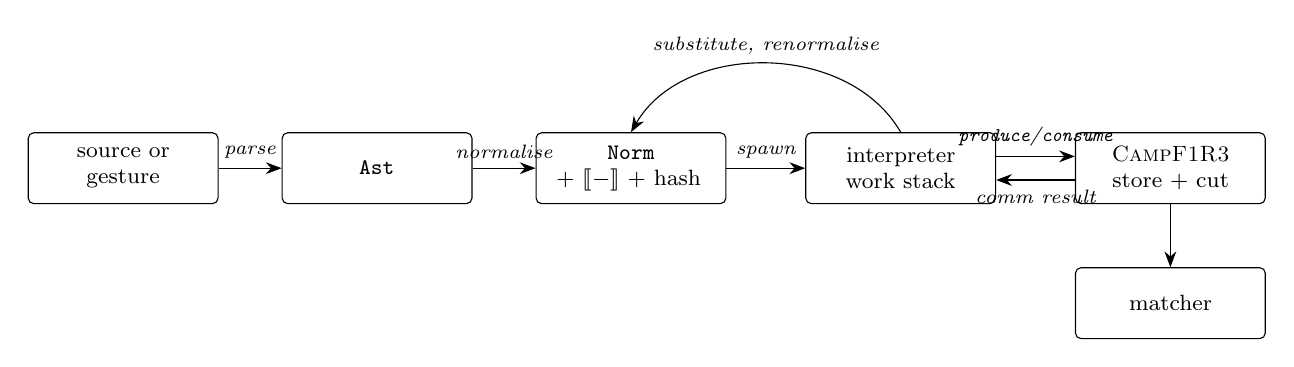
\begin{tikzpicture}[
  st/.style={draw,rounded corners=2pt,align=center,font=\footnotesize,minimum height=9mm,inner sep=3pt,text width=22mm},
  lb/.style={font=\scriptsize\itshape},
  ar/.style={-{Stealth[length=2mm]},thin}]
\node[st] (src) {source or gesture};
\node[st,right=8mm of src] (ast) {\code{Ast}};
\node[st,right=8mm of ast] (norm) {\Norm\\ \footnotesize + $\enc{-}$ + hash};
\node[st,right=10mm of norm] (int) {interpreter\\ \footnotesize work stack};
\node[st,right=10mm of int] (camp) {\Camp\\ \footnotesize store + cut};
\node[st,below=8mm of camp] (match) {matcher};
\draw[ar] (src)--node[lb,above]{parse}(ast);
\draw[ar] (ast)--node[lb,above]{normalise}(norm);
\draw[ar] (norm)--node[lb,above]{spawn}(int);
\draw[ar] ([yshift=1.5mm]int.east)--node[lb,above]{\code{produce}/\code{consume}}([yshift=1.5mm]camp.west);
\draw[ar] ([yshift=-1.5mm]camp.west)--node[lb,below]{comm result}([yshift=-1.5mm]int.east);
\draw[ar] (camp)--(match);
\draw[ar] (int.north) to[out=120,in=60] node[lb,above]{substitute, renormalise} (norm.north);
\end{tikzpicture}
\end{center}

\subsection{The encoding is already a bytecode}\label{sec:already}

The distance between the two options is smaller than the vocabulary suggests.
$\enc{-}$ is a flat byte string in which each constructor is a tag byte followed
by LEB128 lengths and its fields, identifiers never appear, and subterm
encodings are memoised bottom-up and reused as order keys. Compare it with what
a bytecode gives.

\begin{center}
\begin{tabularx}{\linewidth}{@{}l>{\raggedright\arraybackslash}X>{\raggedright\arraybackslash}X@{}}
\toprule
Property & $\enc{\Norm}$ & a conventional bytecode\\
\midrule
Layout & flat byte string, prefix order & flat byte string\\
Dispatch & one tag byte per node (\code{0x00}--\code{0x20}) & one opcode byte\\
Operands & LEB128 lengths, de Bruijn indices & immediates, slot numbers\\
Constants & memoised subterm encodings with 32-byte hashes & constant pool\\
Control flow & \emph{structural}: implicit in the nesting & \emph{explicit}: PC, jumps, blocks\\
Machine state & the interpreter's work stack & operand stack and frames\\
Recoverable as a term & yes; decoding is a function (\Kind{} Prop.~6.9) & not in general\\
Usable as a store key & yes, by construction & only if the compiler is canonical (Prop.~\ref{prop:canon})\\
\bottomrule
\end{tabularx}
\end{center}

\begin{remark}[The real difference]
The two representations differ in exactly two places: whether control flow is
explicit, and whether the form is invertible to a term. The kernel has no
control flow to make explicit (Proposition~\ref{prop:nobranch}), and
invertibility is required by reflection (Proposition~\ref{prop:refl}), by the
store's identity discipline (Section~\ref{sec:identity}) and by the editor. On
both of the two axes that distinguish them, the kernel wants what $\enc{-}$
already provides. The normal form \emph{is} the kernel's bytecode --- with the
advantage that it was designed, specified, proved to decide congruence, and
budgeted, and the further advantage that it did not have to be designed twice.
\end{remark}

\subsection{The case for}

\begin{enumerate}[leftmargin=1.8em,nosep]
\item \textbf{One representation (C2, C6).} Editor, wire, store key, matcher
input, hash preimage and execution all use the same object. There is no
synchronisation problem, no second serialiser, and nothing to keep in step.
\item \textbf{No new semantic object (C1).} The interpreter's states are
multisets of terms and a store state, which is what the calculus's reduction
relation is stated over. The correspondence argument is a simulation over the
same syntax, and the full abstraction obligation of Section~\ref{sec:proof} does
not arise.
\item \textbf{Reflection is free (C3).} \code{Eval} of a name bound to $@Q$
splices $Q$; no compiler, no cache, no eviction policy, no question about
whether two engines agree. Normalisation has already applied $*@P\equiv P$, so
in many cases the splice was performed before the term reached the interpreter.
\item \textbf{The identity discipline is untouched (C2).} Channel hashes are
\Kind's memoised hashes; \Camp's \code{OrderKey}, \code{GroupKey} and
\code{Replay} profiles work over exactly the bytes the specifications say they
work over.
\item \textbf{Smallest and most portable (C5).} One crate, dependent on
\code{k1ndl1ng-norm} and \code{campf1r3-core} and nothing else; no decoder, no
compiler, no constant pool, no additional \code{wasm32} code-size line item.
\item \textbf{Cost accounting fits (C1).} \Camp{} hooks accounting at the zip
and nowhere else, because in the cost-accounted rho calculus the communication
is where resources are debited. An interpreter with no instructions has nothing
to meter that the store does not already meter, and any later per-term charge
can be levied on \code{Norm::size}, which is already exposed.
\item \textbf{Shortest path to phase~5 (C7).} The interpreter is the last piece
before the browser demonstration and the headset executive; Option~B is a crate
of a few hundred lines over an API that already exists.
\end{enumerate}

\subsection{The case against}

Stated without softening, because these are the costs the recommendation has to
cover.

\begin{enumerate}[leftmargin=1.8em,nosep]
\item \textbf{No amortisation across firings.} A persistent continuation is
walked again on every firing, and its structure re-decided each time. This is
Option~A's point~2, and a naive Option~B forfeits it entirely.
\item \textbf{Re-hashing closed channels.} A body that sends on a closed channel
recomputes that channel's encoding and hash on every firing unless something
memoises it. This is Option~A's point~3, and the largest concrete arithmetic
cost in the loop. A naive Option~B forfeits this too.
\item \textbf{Renormalisation after substitution.} Substituting into a body can
change the encodings of parallel components, hence their order, hence their
parents' encodings; and free levels are assigned after ordering, which \Kind{}
records as Obligation~6.11. A naive implementation re-encodes the whole body per
firing, at $O(m+\sum w\log w\cdot s)$.
\item \textbf{No optimisation seam.} Join ordering, hoisting, and any later
peephole work have nowhere natural to live.
\item \textbf{Coarse suspension.} The only stable suspension points are between
store operations. For the kernel this is arguably correct --- \Camp's soft
checkpoints and quiescence invariant are defined at exactly that granularity ---
but a node that wants to bound a deploy at finer resolution cannot.
\item \textbf{The argument expires.} Everything above depends on
Proposition~\ref{prop:nobranch}, which depends on the kernel being the kernel.
\end{enumerate}

\begin{remark}[Items 1--3 are cacheable, and item~3 is incremental]\label{rem:cache}
Items 1, 2 and 3 are the substance of the case against, and none of them
requires a change of representation to address. Items 1 and 2 are memoisation
keyed by the continuation's content hash --- which the store has already
computed and which \Camp{} carries in the comm result. Item~3 is an incremental
recomputation: a substitution invalidates the memoised encoding only of the
ancestors of its substitution sites, together with the ordering at each
parallel composition on those paths. Section~\ref{sec:rec} turns both into
design commitments and Obligation~\ref{obl:incr} records what has to be proved
about the second.
\end{remark}
%======================================================================
\section{The comparison}\label{sec:cmp}

\subsection{Axis by axis}

\begin{center}
\begin{tabularx}{\linewidth}{@{}l>{\raggedright\arraybackslash}X>{\raggedright\arraybackslash}X@{}}
\toprule
& Option~A: bytecode & Option~B: normal form\\
\midrule
C1 Semantic burden & Executive correspondence \emph{plus} full abstraction for
$\cmp{-}$, against an equivalence still being reshaped by the behavioural work &
Executive correspondence only, over the syntax the calculus already uses\\
C2 Identity & Safe only under Decision~\ref{dec:notakey}; canonicity of a
compiler is not inherited (Prop.~\ref{prop:canon}) & Untouched: the executed
object is the hashed object\\
C3 Reflection & Contains a term interpreter or a run-time compiler with a
hash-keyed cache (Prop.~\ref{prop:refl}) & Splice, and normalisation has often
done it already\\
C4 Performance & Addresses structural dispatch only; ceiling set by
Remark~\ref{rem:amdahl}; genuine wins on hot persistent continuations and closed
channels & Forfeits those wins unless they are cached
(Remark~\ref{rem:cache})\\
C5 Budgets & A third crate, a compiler, a decoder, a constant pool; internal
streams only, so a modest fuzz surface & One crate over two existing APIs; no
new representation to keep total\\
C6 Consumers & Headset, browser and node all carry terms anyway, and would carry
code additionally & Every consumer uses the object it already holds\\
C7 Extensibility & Right answer for \code{match}, \code{let}, \code{select},
methods, arithmetic --- none of which exist yet & Correct while
Prop.~\ref{prop:nobranch} holds; must be revisited when it fails\\
\bottomrule
\end{tabularx}
\end{center}

\subsection{The shape of the finding}

Three of the seven axes are not close. C1, C2 and C3 all favour Option~B, and
they do so for the same underlying reason: \emph{in rho, code is data, and this
programme has already paid, carefully, to make that data canonical}. $\enc{-}$
was designed so that congruence is decided by byte equality; \Camp{} was
designed so that identity, ordering, determinism and replay are all consequences
of that encoding. Introducing a second executable representation means either
excluding it from all of that machinery --- in which case it is a cache --- or
re-deriving the machinery for it, which is a large and avoidable proof effort.

C4 is the axis on which Option~A was supposed to win, and
Proposition~\ref{prop:nobranch} takes most of that away: there is no ground
layer to compile, and the compiled form of a kernel continuation is a branchless
list. What remains of C4 --- amortisation and precomputed channel hashes --- is
memoisation, and memoisation does not require an instruction set.

\subsection{The measurement that would settle it}\label{sec:measure}

The argument above is structural, and structural arguments should be given a
way to be wrong.

\begin{requirement}[Instrument the loop]\label{req:measure}
The first interpreter \MUST{} be instrumented to report, per benchmark run, the
fraction of wall time spent in: (i) the matcher; (ii)
\code{k1ndl1ng-norm::substitute}; (iii) re-ordering, re-encoding and hashing;
(iv) \Camp's own bookkeeping; (v) structural dispatch and term walking in the
interpreter; (vi) allocation. The benchmarks \MUST{} include \Camp's
benchmark~1 (single-channel ping-pong) and benchmark~5 (persistent receive with
a produce storm), which between them isolate the loop with and without
amortisation.
\end{requirement}

\begin{decision}[The threshold]\label{dec:threshold}
If category~(v) exceeds 15\% of the loop on either benchmark \emph{after} the
prepared continuation of Section~\ref{sec:plan} is in place, Option~A \MUST{} be
reopened and this note revised. Below that figure it \MUST{} not be, on the
grounds that 15\% is the ceiling on the improvement, \Kind's own regression gate
is 10\%, and a second representation carrying a full abstraction obligation
needs to beat the noise floor by a comfortable margin to be worth it.
\end{decision}

\begin{requirement}[Measure the hypothesis, not only the outcome]
The same instrumentation \MUST{} report two structural statistics over the
corpus: the proportion of channels in continuation bodies that are closed, and
hence hashable once; and the mean proportion of a body's nodes that are
ancestors of a substitution site, and hence need re-encoding per firing. The
first bounds the value of the prepared continuation; the second bounds the value
of incremental renormalisation (Obligation~\ref{obl:incr}).
\end{requirement}

\subsection{What would change the answer}\label{sec:change}

\begin{enumerate}[leftmargin=1.8em,nosep]
\item \textbf{A ground layer.} The moment \code{Expr} arrives --- K2 guards
promoted from feature-gated to routine, or the kernel widened towards full
f1r3lang with \code{match}, \code{let}, \code{select}, collections, methods and
arithmetic --- Proposition~\ref{prop:nobranch} fails, the 1.2 argument returns
in full force, and a stack machine becomes the right answer for the new middle.
Note that it becomes the right answer \emph{for the expression layer}, not
necessarily for the process layer: a hybrid in which processes are interpreted
as terms and expressions are compiled to a stack machine keeps every property
argued for here and gets the dispatch win exactly where there is dispatch to
win. That is the shape the 1.2 design already had.
\item \textbf{Metering moving off the zip.} \Camp{} hooks accounting at the
communication because that is where the cost-accounted calculus debits. If a
future cost model needs to charge per unit of local work at a finer granularity
than a term's size, an instruction counter becomes the natural meter.
\item \textbf{Execution off the CPU.} An FPGA, an accelerator, or the hardware
direction of the wider programme would want a fixed-width instruction word
rather than a pointer graph. This is a compilation target question, and it can
be answered by a compiler from \Norm{} written then, for that target, without
the interpreter having been built around one now.
\item \textbf{Sub-communication suspension.} A requirement to suspend, migrate
or bound a computation between two points \emph{within} a continuation body,
rather than between store operations.
\item \textbf{The measurement.} Decision~\ref{dec:threshold}.
\end{enumerate}

%======================================================================
\section{Recommendation}\label{sec:rec}

\subsection{The decisions}

\begin{decision}[Interpret the normal form]\label{dec:main}
The v1 interpreter \MUST{} execute \Norm{} directly. No bytecode, no compiled
representation and no virtual machine \MUST{} appear between
\code{k1ndl1ng-norm} and \code{campf1r3-core} in v1.
\end{decision}

\begin{decision}[The interpreter is its own crate]\label{dec:crate}
The interpreter \MUST{} be a crate depending only on \code{k1ndl1ng-norm},
\code{campf1r3-core} and the kernel matcher, and \MUSTNOT{} be added to
\code{k1ndl1ng-norm} or to \code{campf1r3-core}, both of which forbid it ---
\Kind{} Requirement~3.6 (``no executive in these crates'') and \Camp's
non-goals. It inherits both families' constraints: no recursion, no
\code{unsafe}, no panics on input-derived data, \code{wasm32} as a first-class
target, and the union of the two dependency allowlists.
\end{decision}

\begin{remark}[A name]
\Kind{} is what you feed a campfire. The component that makes it burn hotter
without changing what is burning is a bellows; \Bell{} is offered as a working
name for the interpreter crate, for the same reason \Kind{} was: the family
should be nameable by someone who has seen one member.
\end{remark}

\subsection{The prepared continuation}\label{sec:plan}

This is where Option~A's real benefits are collected without its costs.

\begin{decision}[Plans, keyed by content hash]\label{dec:plan}
The interpreter \SHOULD{} maintain a bounded cache of \emph{plans}, keyed by the
content hash of a continuation --- which \Camp{} has already computed and which
travels in the comm result. A plan holds, for one continuation body:
\begin{enumerate}[nosep,leftmargin=1.6em]
\item the flattened list of top-level components with their constructors, so the
shape decision of step~4--5 is made once rather than per firing;
\item for each channel occurring in the body, whether it is closed, and if so
its encoding and its 32-byte hash, precomputed;
\item the same for closed argument subterms, which are data that will be sent
unchanged on every firing;
\item the binder slot map: which de Bruijn index each pattern variable occupies,
so building $\sigma$ is an array write rather than a traversal;
\item the set of nodes that are ancestors of a binder occurrence, which is
exactly the set whose encodings a substitution can invalidate.
\end{enumerate}
A plan \MUST{} be derivable from the term alone, \MUST{} be a pure function of
it, and \MUSTNOT{} be observable: two runs differing only in cache occupancy
\MUST{} produce identical results, logs and charges. The last is free under
\Camp's accounting hooks, which fire at the zip and not at local work.
\end{decision}

\begin{remark}[Why this is the whole of Option~A that the kernel can use]
Points 2 and 3 of Section~\ref{sec:A} --- amortisation over persistent
continuations, and compile-time channel identity --- are the two concrete wins a
bytecode would have delivered at the kernel. Both are properties of the
\emph{term}, computed once and reused; neither needs a change of
representation, an instruction set, a program counter or a compiler. What the
plan is, precisely, is the answer to ``what did compilation actually buy?''
with the representation change removed.
\end{remark}

\begin{obligation}[Incremental renormalisation]\label{obl:incr}
Show that after substituting $\sigma$ into a normalised body, the memoised
encodings that require recomputation are exactly those of the ancestors of the
substitution sites, together with the re-ordering of each parallel composition
on those paths and the reassignment of free levels that
\Kind{} Obligation~6.11 already requires; and bound the number of ordering
rounds needed to reach a fixed point. If the bound is not constant, state the
loop and its termination measure. This is the obligation that turns item~3 of
Section~\ref{sec:B}'s case against into a cost proportional to the substitution
rather than to the body.
\end{obligation}

\subsection{The seam}

\begin{decision}[A backend seam, defined at the continuation]\label{dec:seam}
The interpreter \SHOULD{} be written against an internal trait whose unit is a
prepared continuation, not a term node:
\begin{center}\small
\code{trait Backend \{ fn prepare(\&mut self, body: \&Norm) -> PlanId;\\
\hspace*{2.6em} fn run(\&mut self, p: PlanId, sigma: \&Subst, space: \&mut S) -> Result<Vec<Op>>; \}}
\end{center}
so that a compiled backend, if Section~\ref{sec:change} is ever triggered, is an
implementation of \code{Backend} rather than a redesign of the executive. The
seam \MUSTNOT{} appear in any public API of \code{k1ndl1ng-norm} or
\code{campf1r3-core}, and the default backend \MUST{} be the direct one.
\end{decision}

\begin{remark}[Why the seam is at the continuation]
The continuation is the unit that has a content hash, that the store hands back,
that is fired repeatedly, and that a compiler would compile. A seam at the term
node would be a visitor, which constrains the interpreter without giving a
compiler anything to hold; a seam at the whole program would be too coarse to
substitute a backend for hot contracts only.
\end{remark}

\subsection{What this costs the delivery plan}

\Kind's phases~3 and~5 end, respectively, with ``name equality is a hash
comparison'' and ``\Camp{} in a browser runs on real terms instead of
\code{ExactBytes}''. Under Decision~\ref{dec:main} the interpreter is a
phase-5 companion: a crate of a few hundred lines over two APIs that already
exist, gated by the kernel matcher rather than by anything in this note. Under
Option~A it would be a phase of its own, with a compiler, a machine, a decoder,
a differential test between compiled and interpreted execution, and a proof
obligation that the behavioural line is not yet ready to state cleanly. The
recommendation is therefore also the shorter path to the first end-to-end
demonstration on all three executives.

%======================================================================
\section{Summary}

\begin{center}
\begin{tabularx}{\linewidth}{@{}l>{\raggedright\arraybackslash}X@{}}
\toprule
\multicolumn{2}{@{}l}{\textbf{Decisions proposed}}\\
\midrule
\ref{dec:notakey} & A compiled form, if ever introduced, is never a store key, a
wire format or a hash preimage.\\
\ref{dec:threshold} & Reopen Option~A only if structural dispatch exceeds 15\%
of the instrumented loop with plans in place.\\
\ref{dec:main} & The v1 interpreter executes the normal form directly.\\
\ref{dec:crate} & It is its own crate, inheriting both families' constraints.\\
\ref{dec:plan} & It caches prepared continuations keyed by content hash.\\
\ref{dec:seam} & It is written against a backend trait whose unit is a prepared
continuation.\\
\midrule
\multicolumn{2}{@{}l}{\textbf{Obligations and measurement}}\\
\midrule
\ref{obl:incr} & Incremental renormalisation after substitution touches only
ancestors of substitution sites; bound the ordering rounds.\\
\ref{req:measure} & Instrument the loop; report the six-way split and the two
structural statistics.\\
\midrule
\multicolumn{2}{@{}l}{\textbf{Open for review}}\\
\midrule
1 & Whether the hybrid of Section~\ref{sec:change}(1) --- terms interpreted,
expressions compiled --- should be the stated long-run architecture now, so that
K2 lands into a shape that was planned rather than discovered.\\
2 & Whether the interpreter crate belongs in the \Kind{} workspace, the \Camp{}
repository, or its own; this note assumes its own, on the grounds that it is the
only component that depends on both.\\
3 & The name.\\
\bottomrule
\end{tabularx}
\end{center}

\noindent
The one-sentence version: the kernel's bytecode already exists, it is called
$\enc{-}$, it was specified for other reasons and it is better than a bytecode
designed now would be, because it is invertible, canonical, hashed and already
what the store, the wire and the editor speak --- and the only thing a real
bytecode would have added at this scale is memoisation, which can be had
without it.

\bigskip
\noindent\rule{\linewidth}{0.4pt}\\[2pt]
\footnotesize
Sources, all read on 17 September 2026: \code{campf1r3-spec.tex} (v0.1) and
\code{k1ndl1ng-spec.tex} (v0.2) in \code{publications/campf1r3}; the March 2026
architecture for a rholang~1.2 bytecode interpreter and its full abstraction
proof sketch; \emph{Rhobots in Space}; and
\code{denotational-semantics-for-rho/knot-rho.tex}.

\end{document}
